\documentclass{jarticle}
\usepackage[dvips]{graphicx}

\begin{document}

\begin{center}
{\LARGE \bf Plamo Linux へようこそ!!}
\end{center}

\vspace{1cm}

\section{Mule + YaTeX + xdvi のテスト}

この文書を mule で開いてください。自動的に YaTeX が起動して、
\verb+\section+ や \verb+\begin .. \end+ など、LaTeX のコマンド部の色が
変って表示されているでしょう。

次に、C-c, t, j を押して、TeX でコンパイルしてください。YaTeX が自動的
に別の窓を開いて、この文書を pTeX でコンパイルしてくれます。

次に C-c, t, p を押して、xdvi を使って、DVI ファイルをプレビューします。
このファイルには、EPSF ファイルが含まれているので、正しくインストールで
きていれば、xdvi が ghostcript を起動して、グラフ部分も表示されるはずで
す。

\begin{figure}[hb]
\begin{center}

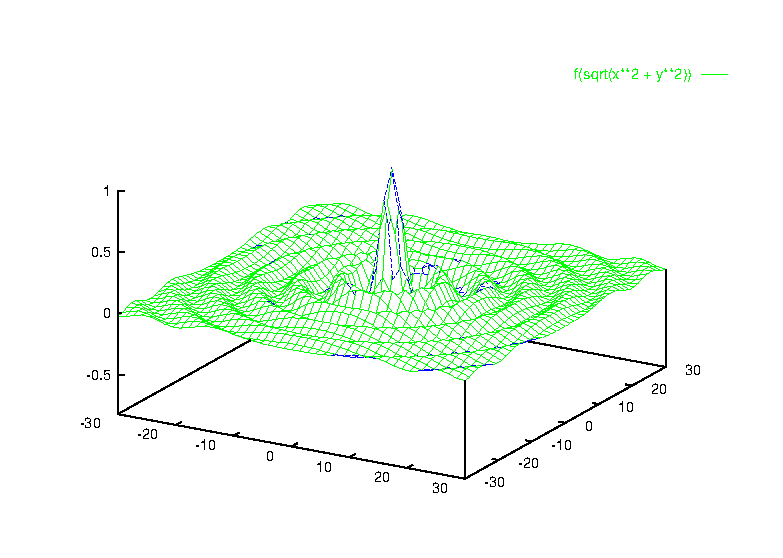
\includegraphics{gnuplot-demo.eps}
\caption{GNUPLOT で書いた 3 次元グラフ}
\label{figdemo}

\end{center}
\end{figure}


図 \ref{figdemo} は GNUPLOT を使って、
\[
f(x) = \frac{\sin (x)}{x}
\]
を描いてみました。

次に C-c, t, l を押して、dvips を起動して DVI ファイルを PS ファイルに
変換してみます。プリンタの設定が済んでいれば、PostScript プリンタの名前
を lpr -Pps のように指定して、プリンタに送ってみます。プリンタの設定をし
ていない場合、``$|$ lpr'' の部分は ``$>$ texdemo.ps'' と修正して、ファイル
に書きだし、gv を起動して、texdemo.ps という PostScript ファイルが正しく
できているかを確認してください。

\end{document}
